%%%%%%%%%%%%%%%%%%%%%%%%%%%%%%%%%%%%%%%%%%%%%%%%%%%%%%%%%%%%%%%%%%%%%%%%%%%%%%%%
\documentclass[11pt]{article} % Dokumentenklasse

\usepackage[utf8]{inputenc} % Textkodierung: UTF-8
\usepackage[T1]{fontenc} % Zeichensatzkodierung

\usepackage[USenglish]{babel}% http://ctan.org/pkg/babel
\usepackage{graphicx} % Grafiken
\usepackage[absolute]{textpos} % Positionierung

% Schriftart Helvetica:
\usepackage[scaled]{helvet}
\renewcommand{\familydefault}{\sfdefault}

\usepackage{calc} % Berechnungen
\usepackage{tabto} % Tabulatoren
\usepackage{parskip}

\usepackage{enumitem}

% Debugging:
%\usepackage{layout} % Layout-Informationen
%\usepackage{printlen} % Längenwerte ausgeben

%%%%%%%%%%%%%%%%%%%%%%%%%%%%%%%%%%%%%%%%%%%%%%%%%%%%%%%%%%%%%%%%%%%%%%%%%%%%%%%%
% EINSTELLUNGEN
%%%%%%%%%%%%%%%%%%%%%%%%%%%%%%%%%%%%%%%%%%%%%%%%%%%%%%%%%%%%%%%%%%%%%%%%%%%%%%%%

% Seitenränder:
\newcommand{\SeitenrandOben}{43.5mm}
\newcommand{\SeitenrandRechts}{20mm}
\newcommand{\SeitenrandLinks}{20mm}
\newcommand{\SeitenrandUnten}{10mm}

\newcommand{\UniversitaetLogoBreite}{19mm}
\newcommand{\UniversitaetLogoHoehe}{1cm}

\usepackage[a4paper,
top=\SeitenrandOben,
bottom=\SeitenrandUnten,
inner=\SeitenrandLinks,
outer=\SeitenrandRechts,
foot=0cm,
head=0cm
]{geometry}

\textblockorigin{\SeitenrandLinks}{\SeitenrandOben} % Ursprung für Positionierung

\setlength{\parindent}{0pt}
%\setlength{\baselineskip}{32pt}
\setlength{\parskip}{\baselineskip}
\TabPositions{4cm}
\pagestyle{empty}

%%%%%%%%%%%%%%%%%%%%%%%%%%%%%%%%%%%%%%%%%%%%%%%%%%%%%%%%%%%%%%%%%%%%%%%%%%%%%%%%
% General stuff
%%%%%%%%%%%%%%%%%%%%%%%%%%%%%%%%%%%%%%%%%%%%%%%%%%%%%%%%%%%%%%%%%%%%%%%%%%%%%%%%
\newcommand{\Problem}[1]{\paragraph*{Problem #1:}\qquad}
\newcommand{\Topic}[1]{
	\newpage
	\section*{#1}}

\newcommand{\Given}{\textbf{Given:\qquad\qquad}}
\newcommand{\Searched}{\textbf{Searched:\qquad}}
\newcommand{\Solution}{\textbf{Solution:\qquad}}

%%%%%%%%%%%%%%%%%%%%%%%%%%%%%%%%%%%%%%%%%%%%%%%%%%%%%%%%%%%%%%%%%%%%%%%%%%%%%%%%
% Math stuff
%%%%%%%%%%%%%%%%%%%%%%%%%%%%%%%%%%%%%%%%%%%%%%%%%%%%%%%%%%%%%%%%%%%%%%%%%%%%%%%%
\usepackage{amsmath}
\usepackage{amssymb}

\newcommand{\R}{\mathbb{R}}
\newcommand{\Vector}[1]{\R^{#1}}
\newcommand{\Matrix}[2]{\R^{#1 \times #2}} % !!! DON'T TOUCH !!!
%%%%%%%%%%%%%%%%%%%%%%%%%%%%%%%%%%%%%%%%%%%%%%%%%%%%%%%%%%%%%%%%%%%%%%%%%%%%%%%%


\newcommand{\ExerciseNumber}{07}

\newcommand{\PersonOne}{Marcel Bruckner (03674122)}
\newcommand{\PersonTwo}{Julian Hohenadel (03673879)}
\newcommand{\PersonThree}{Kevin Bein (03707775)}


%%%%%%%%%%%%%%%%%%%%%%%%%%%%%%%%%%%%%%%%%%%%%%%%%%%%%%%%%%%%%%%%%%%%%%%%%%%%%%%%
% DOKUMENT
%%%%%%%%%%%%%%%%%%%%%%%%%%%%%%%%%%%%%%%%%%%%%%%%%%%%%%%%%%%%%%%%%%%%%%%%%%%%%%%%

\begin{document}

%%%%%%%%%%%%%%%%%%%%%%%%%%%%%%%%%%%%%%%%%%%%%%%%%%%%%%%%%%%%%%%%%%%%%%%%%%%%%%%%
\begin{textblock*}{\UniversitaetLogoBreite}[1,0](\textwidth-1mm, 2cm-\SeitenrandOben)%
	\raggedleft
\includegraphics{../Ressources/Universitaet_Logo_RGB.pdf}%
\end{textblock*}


\begin{textblock*}{\textwidth}[0,0](0cm, 0cm)%
	{\fontsize{24pt}{26pt}\selectfont\textbf{Exercise}}
	
	\vspace*{14pt}
	{\fontsize{18pt}{27pt}\selectfont\textbf{\ExerciseNumber}}
\end{textblock*}

\vspace*{92.2mm}
\fontsize{15pt}{17.5pt}\selectfont%
TUM Department of Informatics

\renewcommand{\baselinestretch}{1.47}
\normalsize\selectfont
\vspace*{17.1mm}
\textbf{Supervised by}\tab
\begin{minipage}[t]{\textwidth-\CurrentLineWidth}
	Prof. Dr. Stephan Günnemann\\
	Informatics 3 - Professorship of Data Mining and Analytics\strut
\end{minipage}

\vspace*{4.3mm}
\textbf{Submitted by}\tab
\begin{minipage}[t]{\textwidth-\CurrentLineWidth}
	\PersonOne\\
	\PersonTwo\\
	\PersonThree
\end{minipage}

\vspace*{-1mm}
\textbf{Submission date}\tab 
\begin{minipage}[t]{\textwidth-\CurrentLineWidth}
	Munich, \today
\end{minipage}
\newpage % !!! DON'T TOUCH !!!
%%%%%%%%%%%%%%%%%%%%%%%%%%%%%%%%%%%%%%%%%%%%%%%%%%%%%%%%%%%%%%%%%%%%%%%%%%%%%%%%

%%%%%%%%%%%%%%%%%%%%%%%%%%%%%%%%%%%%%%%%%%%%%%%%%%%%%%%%%%%%%%%%%%%%%%%%%%%%%%%%
% !!! HOMEWORK STARTS HERE !!!
%%%%%%%%%%%%%%%%%%%%%%%%%%%%%%%%%%%%%%%%%%%%%%%%%%%%%%%%%%%%%%%%%%%%%%%%%%%%%%%%
%
\Topic{Constrained Optimization}
%
\Problem{1}
%
\begin{flushleft}
Constraints:\\
\begin{align}
\theta_1 + \theta_2 \leq 12 &\implies \theta_2 \leq 12 - \theta_1\\
- \theta_1 + 2\theta_2 \geq -3 &\implies \theta_2 \geq \frac{\theta_1-3}{2}\\
- 5\theta_1 + 3\theta_2 \leq -4 &\implies \theta_2 \leq \frac{1}{3}(5\theta_1-4)\\
\theta_2 \geq 2\\
\theta_1 \geq 2
\end{align}
Plot: Axis along $x$-dimension: $\theta_1$, Axis along $y$-dimension: $\theta_2$, simply plot the functions (1) up to (5):
\begin{align*}
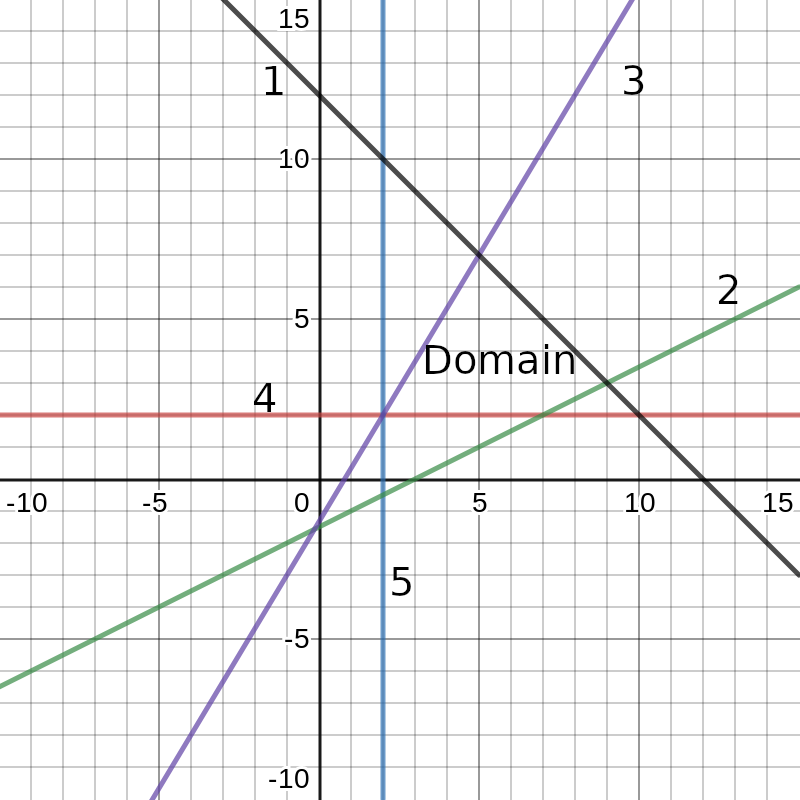
\includegraphics[scale=0.3]{graphs/graph_1.png}
\end{align*}
$f(\theta)=2\theta_1 -3\theta_2$ Minimizer and maximizer both need to be a corner vertex of the domain.\\
Simple testing against $(2,2)$, $(7,2)$, $(9,3)$ and $(5,7)$ shows the solution:\\
Minimizer $\theta_{min} = (5,7) f(\theta_{min})= -11$\\
Maximizer $\theta_{max} = (9,3) f(\theta_{max})= 9$\\
\end{flushleft}
%
%
\Problem{2}
%
\begin{flushleft}
a)\\
Constraints:\\
\begin{align*}
\theta_1 + \theta_2 \leq 4\qquad \qquad(1)\\
0 \leq \theta_1 \leq 3\qquad \qquad(2)\\
0 \leq \theta_2 \leq 2.5\qquad \qquad(3)
\end{align*}
Plot: Axis along $x$-dimension: $\theta_1$, Axis along $y$-dimension: $\theta_2$, simply plot the functions (1) up to (3):
\begin{align*}
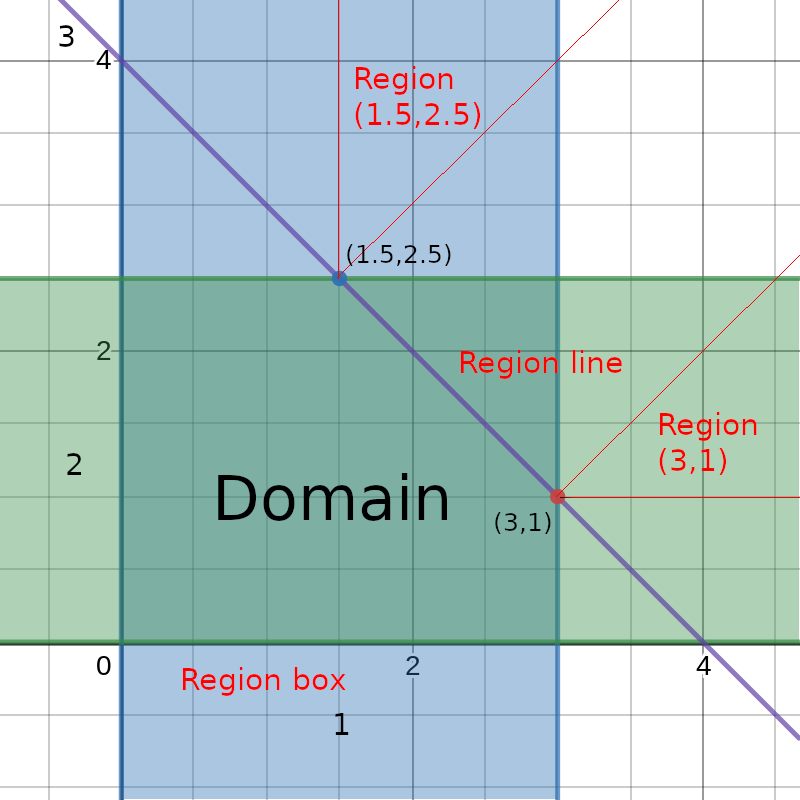
\includegraphics[scale=0.3]{graphs/graph_2.png}
\end{align*}
Domain corner vertices: $(0,0)$, $(3,0)$, $(3,1)$, $(1.5,2.5)$, $(0,2.5)$\\
Domain regions: Domain (inside), box, line, $(3,1)$, $(1.5,2.5)$\\
\begin{align*}
\pi_\mathcal{X}(p) &= p \text{ if } p \in \text{ Domain (inside)}\\
\pi_\mathcal{X}(p) &= (3,1) \text{ if } p \in \text{ Region (3,1) }\\
\pi_\mathcal{X}(p) &= (1.5,2.5) \text{ if } p \in \text{ Region (1.5,2.5)}\\
\pi_\mathcal{X}(p) &= \pi_{line} \text{ if } p \in \text{ Region line}\\
\pi_\mathcal{X}(p) &= \pi_{box} \text{ if } p \in \text{ Region box}\\
\end{align*}
\begin{align*}
p \in \text{ Domain (inside)} &= \{p | p \in \mathcal{X}\}\\
p \in \text{ Region (3,1) } &= \{p | p_2 \geq 1 \land -p_1 + p_2 \leq -2\}\\
p \in \text{ Region (1.5,2.5)} &= \{p | p_1  \geq 1.5 \land -p_1+p_2 \geq 1\}\\
p \in \text{ Region line} &= \{p | p_1 +p_2 > 4 \land -2 < -p_1+p_2 < 1\}\\
p \in \text{ Region box} &= \{p | p \notin \mathcal{X} \land (p_1 < 1.5 \lor p_2 < 1)\}\\
\end{align*}
Let $a$ be $(4,0)$ and let $b$ be $(0,4)$:\\ 
\begin{align*}
\pi_{line}(p) &= a + \frac{(p-a)^{T}(b-a)}{||b-a||^{2}_{2}}(b-a)\\
&= \begin{pmatrix}4\\0\end{pmatrix} + \frac{(p_1-4, p_2)\begin{pmatrix}-4\\4\end{pmatrix}}{32} \begin{pmatrix}-4\\4\end{pmatrix}\\
&= \begin{pmatrix}4\\0\end{pmatrix} + \frac{16-4p_1+4p_2}{32} \begin{pmatrix}-4\\4\end{pmatrix}\\
&= \begin{pmatrix}4\\0\end{pmatrix} + \begin{pmatrix}2-\frac{1}{2}p_1+\frac{1}{2}p_2\end{pmatrix} \begin{pmatrix}-1\\1\end{pmatrix}\\
&=\begin{pmatrix}2+\frac{1}{2}p_1-\frac{1}{2}p_2\\2-\frac{1}{2}p_1+\frac{1}{2}p_2\end{pmatrix}
\end{align*}
Formula taken from the lecture:
\begin{align*}
\pi_{box}(p) &= \begin{pmatrix}max(0, min(3, p_1))\\max(0, min(2.5, p_2))\end{pmatrix}
\end{align*}
\end{flushleft}
%
%
\Problem{3}
%

%
%
\Problem{4}
%

%
%
%%%%%%%%%%%%%%%%%%%%%%%%%%%%%%%%%%%%%%%%%%%%%%%%%%%%%%%%%%%%%%%%%%%%%%%%%%%%%%%%
% !!! HOMEWORK ENDS HERE !!!
%%%%%%%%%%%%%%%%%%%%%%%%%%%%%%%%%%%%%%%%%%%%%%%%%%%%%%%%%%%%%%%%%%%%%%%%%%%%%%%%

%%%%%%%%%%%%%%%%%%%%%%%%%%%%%%%%%%%%%%%%%%%%%%%%%%%%%%%%%%%%%%%%%%%%%%%%%%%%%%%%
\newpage

\vspace*{-15.8mm}
\fontsize{19pt}{21pt}\selectfont

\vspace{25.3mm}
Appendix

\normalsize\selectfont
\vspace{13.2mm}
We confirm that the submitted solution is original work and was written by us without further assistance. Appropriate credit has been given where reference has been made to the work of others.

\vspace{18.1mm}
\rule[-3.7mm]{\linewidth}{0.5pt}
Munich, \today, Signature \PersonOne

\vspace{18.1mm}
\rule[-3.7mm]{\linewidth}{0.5pt}
Munich, \today, Signature \PersonTwo

\vspace{18.1mm}
\rule[-3.7mm]{\linewidth}{0.5pt}
Munich, \today, Signature \PersonThree
 % !!! DON'T TOUCH !!!
%%%%%%%%%%%%%%%%%%%%%%%%%%%%%%%%%%%%%%%%%%%%%%%%%%%%%%%%%%%%%%%%%%%%%%%%%%%%%%%%

\end{document}
